\chapter{Prompt Engineering}


Prompt engineering is the process of designing and refining
instructions and contextual information to guide a pre-trained
language model towards a desired output, without modifying its
parameters.

\begin{flushleft}
  \begin{minipage}{0.65\linewidth}

    \textbf{Prompts} are sequences of instructions and context that are provided
    as input to a Language Model, to achieve a desired task

    Prompt Engineering is the practice of developing and optimizing
    prompts, to efficiently use LMs for various applications


  \end{minipage}%
  \hfill
  \begin{minipage}{0.3\linewidth}
    \centering
    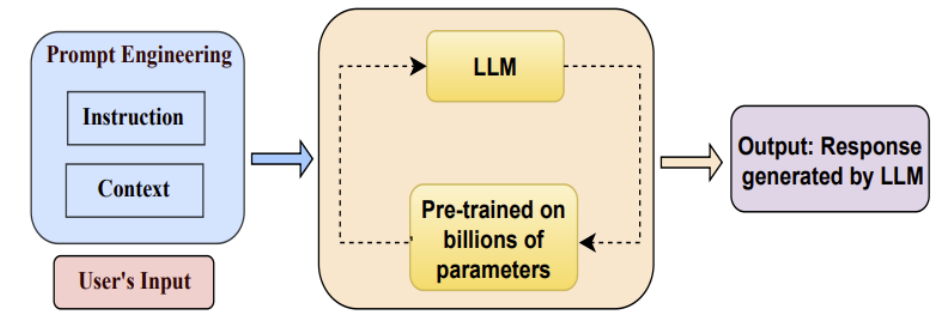
\includegraphics[width=1\linewidth]{content/Parts/images/2026-11-11-11-24-28.png}
  \end{minipage}
\end{flushleft}

\subsection{Prompt Engineering: Main principles}

\begin{itemize}
  \item  \textbf{Specificness}: the more the prompt is specific, the more focused
        output will be obtained
  \item  \textbf{Step-wise approach}: break large tasks into small chunks
  \item \textbf{Iterate and improve}: re-work the inputs with iterative interaction
        with the LM
\end{itemize}

\subsection{What makes a good prompt}

\begin{itemize}
  \item Clearly describe the task to be performed
  \item Provide relevant context and information
  \item Include examples when useful
  \item Specify the expected output format
  \item Define constraints and requirements
  \item Iteratively refine and evaluate the prompt
\end{itemize}

Learning prompt engineering is important for research and advancement of the practice.
Also important for evaluation od limitations od LLMs and they enale innvative applications on top of LLMs.

\section{A basic prompt}




\begin{flushleft}
  \begin{minipage}{0.65\linewidth}

    A prompt is composed with the following components:

    \begin{itemize}
      \item Instructions
      \item Context
      \item Input data
      \item Output indicator
    \end{itemize}
  \end{minipage}%
  \hfill
  \begin{minipage}{0.3\linewidth}
    \centering
    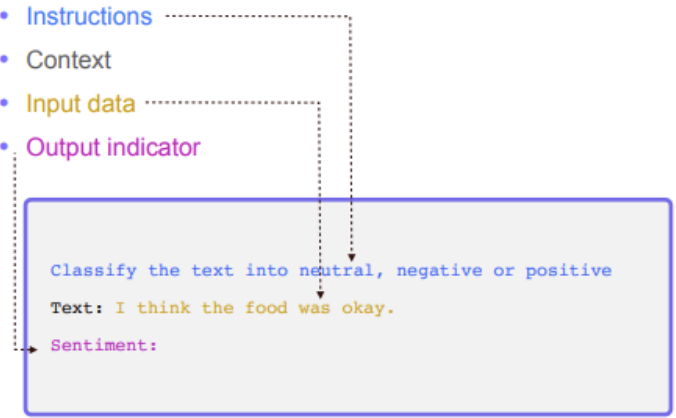
\includegraphics[width=1\linewidth]{content/Parts/images/2026-11-11-11-28-54.png}
  \end{minipage}
\end{flushleft}

\section{New Tasks}

\subsection{Priming}

The practice of providing some initial input to the model before
generating a response. The initial input is intended to guide the model toward generating a more
coherent response

\begin{itemize}
  \item \textbf{ Without priming}: "Write a story about a detective solving a mystery."
  \item  \textbf{With priming}: "Imagine a world where technology is advanced, and detectives use futuristic gadgets to solve crimes. The city is filled with neon lights and towering skyscrapers, creating a cyberpunk atmosphere. The detective in this story is known for his sharp mind and unorthodox methods. He's tasked with solving a mystery involving a missing scientist and a powerful corporation hiding dark secrets."
\end{itemize}


\begin{flushleft}
  \begin{minipage}{0.65\linewidth}
    \subsection{Tabular format prompting}
    Use tabular format for clear organization and presentation of data. Makes it easier for the user to analyze and comprehend the output


  \end{minipage}%
  \hfill
  \begin{minipage}{0.3\linewidth}
    \centering
    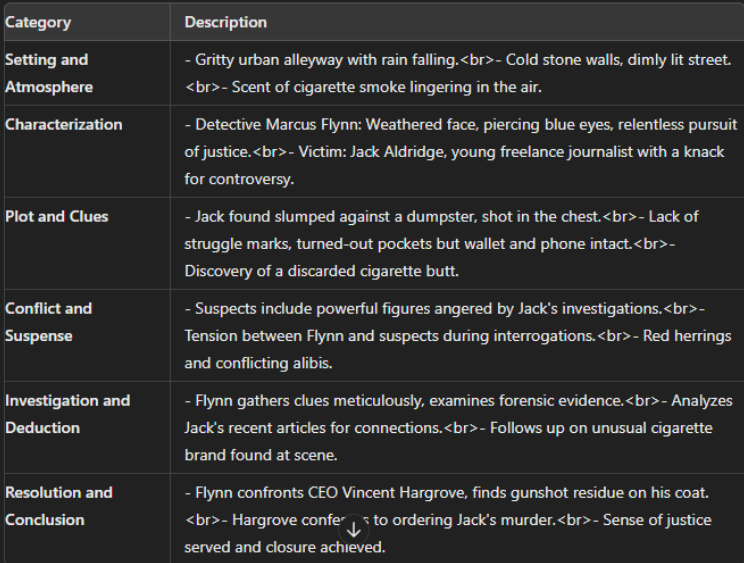
\includegraphics[width=0.7\linewidth]{content/Parts/images/2026-11-11-11-33-13.png}
  \end{minipage}
\end{flushleft}

\subsection{Fill-in-the-blank Prompting}
A prompting technique in which the model is asked to complete
missing parts of a partially specified text or structure.
The provided content guides the model towards producing a
completion consistent with the surrounding information.

"Fill in the placeholders in the following story outline, then write the
completed story.


Create a story about a detective in [choose a setting: e.g., a futuristic city, a
    small coastal town, a bustling international airport]. The detective, [choose
    a name for the detective], is known for [describe a characteristic or skill:
    e.g., keen observation skills, a knack for technology]. The story begins with
  [set the scene: e.g., an unusual disappearance, a cryptic message left
    behind]. As [detective's name] delves into the case, they use [mention a
    tool or method: e.g., advanced gadgets, old-fashioned deduction] to
uncover clues. Through [describe a key location or detail in the
    investigation], [detective's name] discovers [reveal a twist or critical piece
    of information]. However, they face [introduce a challenge or obstacle: e.g.,
    a powerful adversary, a race against time]. How does [detective's name]
navigate this situation? Tell the story of how they solve the mystery."

\subsection{Perspective prompting}
To provide a more comprehensive view of the topic at hand. This
helps in making more informed decisions and have a wider
understanding of a complex issue

\begin{itemize}
  \item  \textbf{Singular perspective}: "Please write about [topic] from the
        perspective of [view point]."
  \item  \textbf{Multiple perspectives}: "Please write an argument [for/against]
        the topic of [topic] from multiple diverse perspectives. Include the names and
        points of view of the different perspectives, such as [view points]"
\end{itemize}


\subsection{Role, Result, Goal, Context, Constraint}


\begin{itemize}
  \item Role: LM's persona $\to$ "You are tasked with writing a compelling
        narrative about a detective who embarks on a mission to uncover the truth
        behind a perplexing mystery."

  \item Result: desired output $\to$ "As the story progresses, reveal how the
        detective meticulously pieces together the evidence, confronts suspects, and
        unravels the hidden motives behind the crime."

  \item Goal: purpose of the output $\to$ "Your objective is to engage the
        reader with a gripping tale that revolves around the detective's journey from
        initial discovery to solving the intricate puzzle."

  \item Context: who, what, where, why $\to$ "The story is set in a bustling
        city where a prominent public figure has been found murdered in their home,
        leaving behind cryptic clues that point to a web of deceit."

  \item Constraint: limitations and guidelines $\to$ "Despite facing numerous
        red herrings and conflicting testimonies, ensure the narrative maintains
        suspense and coherence, leading to a satisfying resolution that ties all loose
        ends."
\end{itemize}

\subsection{I want you to act as prompting}
A robust and universal structure that optimizes the framing of the LM:

\begin{itemize}
  \item I want you to act as…
  \item I  will give you…
  \item You will then…
  \item In a tone / style…
  \item The important details are…
  \item [refine the ouputs as needed]
\end{itemize}



\subsection{Shot prompting}

\begin{itemize}
  \item Zero-shot: No input-output examples are provided. The model
        performs the task based on the instructions.

  \item One-shot: One input-output example is provided to demonstrate the
        expected behaviour.

  \item Few-shot: Multiple input-output examples are provided to guide the
        model towards the expected behaviour.
\end{itemize}

\subsubsection{Zero-shot prompting}
The model receives a task description without additional data.
The model leverages its pre-existing knowledge to generate results
based on the given prompt.

\subsubsection{Few-shot prompting}
Provide the models with a few input-output examples to induce an
understanding of a given task.
Careful prompt-engineering is critical to achieve optimal performance
and mitigate unintended added biases.
One-shot: provide a single example

\paragraph{Example of one/few-shot prompting:}

"Example Story: In the sprawling metropolis of Neo-Tokyo, Detective Alex Hunter
navigated the neon-lit streets with his AI-enhanced glasses. The city buzzed
with holographic advertisements and autonomous vehicles. A renowned scientist
had vanished, leaving behind a trail of encrypted messages. Alex used his
advanced gadgets and unconventional tactics to infiltrate the headquarters of
CyberCorp, a mega-corporation suspected of foul play. Amidst layers of deceit
and high-tech security, he uncovered a conspiracy that threatened the very
fabric of society.

  [add other examples for few-shot prompting]

Task: Now, write a story about a detective solving a mystery."


\subsection{Generate Knowledge Prompting}


\begin{flushleft}
  \begin{minipage}{0.65\linewidth}
    The technique involves using additional knowledge, provided as part
    of the context, to improve results on complex tasks such as
    commonsense reasoning.
    The knowledge used in the context is generated by another model,
    and used in the prompt to make a prediction.
    The highest confidence prediction is then useds

  \end{minipage}%
  \hfill
  \begin{minipage}{0.3\linewidth}
    \centering
    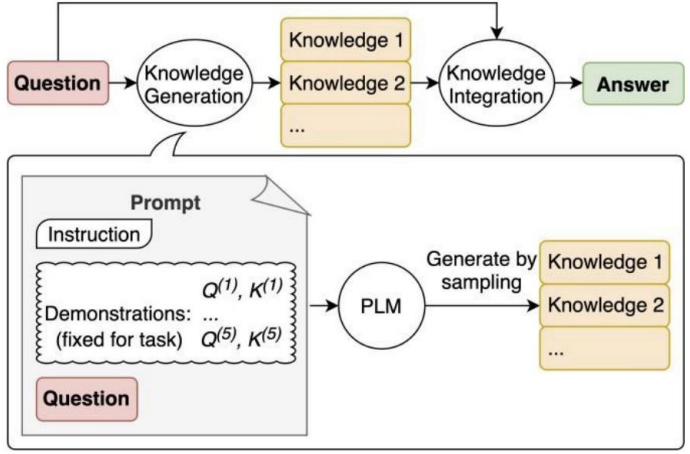
\includegraphics[width=1\linewidth]{content/Parts/images/2026-11-11-11-47-37.png}
  \end{minipage}
\end{flushleft}

\begin{flushleft}
  \begin{minipage}[t]{0.49\linewidth}
    \raggedright


    \begin{tcolorbox}

      Input: Greece is larger than mexico.
      Knowledge: Greece is approximately 131,957 sq km, while Mexico is
      approximately 1,964, 375 sq km, making Mexico 1,389\% larger than Greece.

      Input: A rock is the same size as a pebble.
      Knowledge: A pebble is a clast of rock with a particle size of 4 to 64
      millimetres based on the Udden-Wentworth scale of sedimentology. Pebbles
      are generally considered larger than granules (2 to 4 millimetres
      diameter) and smaller than cobbles (64 to 256 millimetres diameter).

      Input: Part of golf is trying to get a higher point total than others.
      Knowledge:
    \end{tcolorbox}


    \begin{tcolorbox}[title=Knowledge 1]
      The objective of golf is to play a set of holes in the least number of strokes. A
      round of golf typically consists of 18 holes. Each hole is played once in the
      round on a standard golf course. Each stroke is counted as one point, and the
      total number of strokes is used to determine the winner of the game.
    \end{tcolorbox}


    \begin{tcolorbox}[title=Knowledge 2]
      Golf is a precision club-and-ball sport in which competing players (or golfers)
      use many types of clubs to hit balls into a series of holes on a course using the
      fewest number of strokes. The goal is to complete the course with the lowest
      score, which is calculated by adding up the total number of strokes taken on each
      hole. The player with the lowest score wins the game.
    \end{tcolorbox}


  \end{minipage}%
  \hfill
  \begin{minipage}[t]{0.49\linewidth}
    \raggedright
    \begin{tcolorbox}[
        title=High-confidence prediction,
        colframe=green!55!black,    % Verde scuro ed elegante per bordo e titolo
        colback=green!5!white       % Sfondo verdino molto tenue per la leggibilità
      ]
      Question: Part of golf is trying to get a higher point total than others.
      Yes or No?

      Knowledge: The objective of golf is ...

      Explain and Answer: No, the objective of golf is not to get a higher
      point total than others. Rather, the objective is to play a set of holes
      in the least number of strokes. The total number of strokes is used to
      determine the winner of the game, not the total number of points.
    \end{tcolorbox}


    \begin{tcolorbox}[
        title=Low-confidence prediction,
        colframe=red!65!black,      % Rosso mattone/bordeaux non troppo acceso
        colback=red!5!white         % Sfondo rosato molto tenue
      ]
      Question: Part of golf is trying to get a higher point total than others.
      Yes or No?

      Knowledge: Golf is a precision club-and-ball sport in which competing
      players (or golfers) use many types of clubs to hit balls into ...

      Explain and Answer: Yes, part of golf is trying to get a higher point
      total than others. Each player tries to complete the course with the
      lowest score, which is calculated by adding up the total number of
      strokes taken on each hole. The player with the lowest score wins the
      game.
    \end{tcolorbox}
  \end{minipage}
\end{flushleft}


\section{Reasoning and logic}

\subsection{Chain of Thought prompting}

\begin{flushleft}
  \begin{minipage}{0.65\linewidth}

    Chain-of-Thought (CoT) prompting encourages language models to
    produce intermediate reasoning steps before generating a final
    answer.
    In its original formulation, the prompt contains examples that
    demonstrate both the reasoning process and the expected answer.
    CoT is particularly useful for tasks requiring multi-step reasoning,
    such as arithmetic, logical reasoning, and complex problem-solving.s

  \end{minipage}%
  \hfill
  \begin{minipage}{0.3\linewidth}
    \centering
    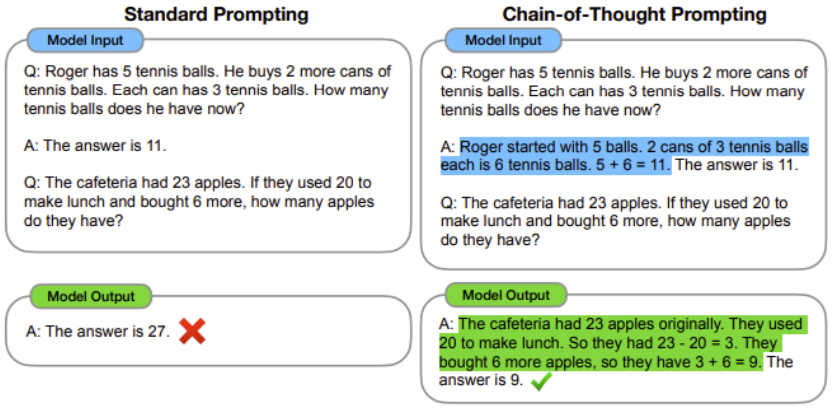
\includegraphics[width=1\linewidth]{content/Parts/images/2026-11-11-12-03-55.png}
  \end{minipage}
\end{flushleft}

\subsubsection{Chain of Thought}


\begin{flushleft}
  \begin{minipage}{0.65\linewidth}
    CoT was proposed to solve challenging
    math problems.

    Examples of solve rate for math
    problems from three repositories.

  \end{minipage}%
  \hfill
  \begin{minipage}{0.3\linewidth}
    \centering
    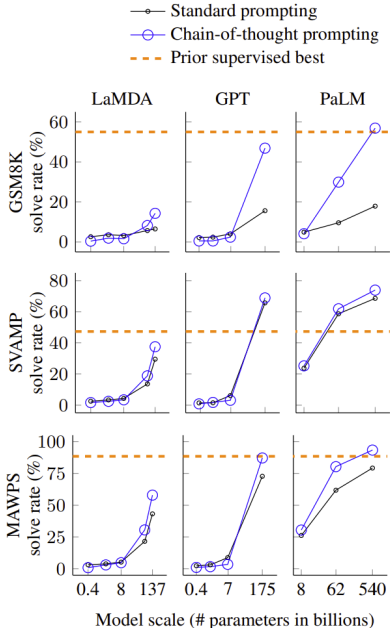
\includegraphics[width=1\linewidth]{content/Parts/images/2026-11-11-12-04-45.png}
  \end{minipage}
\end{flushleft}

\subsection{Self Consistency with CoT (CoT-SC)}

\begin{flushleft}
  \begin{minipage}{0.65\linewidth}
    Self-consistency generates multiple reasoning paths for the same
    problem instead of relying on a single response.

    The final answer is selected by aggregating the answers obtained
    from these different reasoning paths, typically through majority
    voting.
    This technique can improve performance on tasks involving complex
    reasoning.

  \end{minipage}%
  \hfill
  \begin{minipage}{0.3\linewidth}
    \centering
    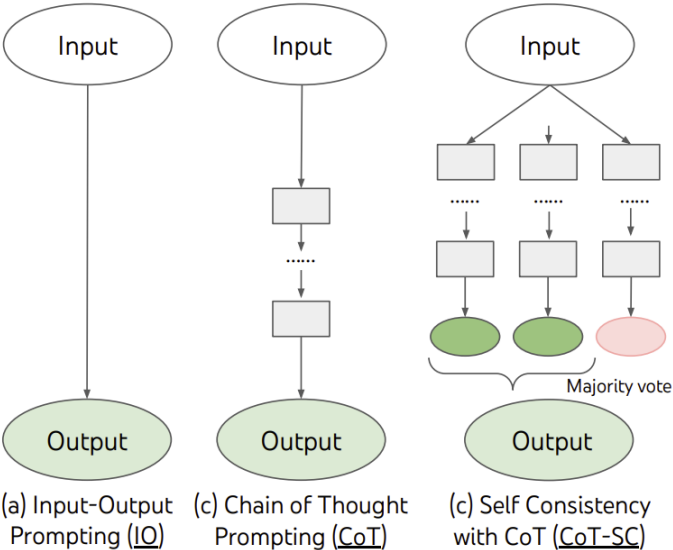
\includegraphics[width=1\linewidth]{content/Parts/images/2026-11-11-12-05-44.png}
  \end{minipage}
\end{flushleft}